\documentclass[a4paper, 12pt]{article}%тип документа



%отступы
\usepackage[left=1cm,right=1cm,top=1cm,bottom=2cm,bindingoffset=0cm]{geometry}

%%% Работа с русским языком
\usepackage{graphicx}
\usepackage{cmap}                           % поиск в PDF
\usepackage{mathtext} 			 	       % русские буквы в формулах
\usepackage[T2A]{fontenc}               % кодировка
\usepackage[utf8]{inputenc}              % кодировка исходного текста
\usepackage[english,russian]{babel} 
\usepackage{float}

\usepackage[export]{adjustbox} % локализация и переносы

\usepackage{subfig}% http://ctan.org/pkg/subfig
\usepackage{booktabs}

\usepackage{wrapfig}


%Матеша
\usepackage{amsmath,amsfonts,amssymb,amsthm,mathtools} % AMS
\usepackage{icomma} % "Умная" запятая

%\mathtoolsset{showonlyrefs=true} % Показывать номера только у тех формул, на которые есть \eqref{} в тексте.

%% Шрифты
\usepackage{euscript}	 % Шрифт Евклид
\usepackage{mathrsfs} % Красивый матшрифт

%% Свои команды
\DeclareMathOperator{\sgn}{\mathop{sgn}}

%% Перенос знаков в формулах (по Львовскому)
\newcommand*{\hm}[1]{#1\nobreak\discretionary{}
	{\hbox{$\mathsurround=0pt #1$}}{}}




\author{Гаврилин Илья Дмитриевич \\
	Б01-101}
\title{\textbf{Работа 3.2.1 \\ 
		сдвиг фаз в цепи переменного тока}}
	
\begin{document}
	\maketitle
	\section{Аннотация}
	В ходе работы производятся измерения зависимости сдвига фаз в RC, RL-цепи от сопротивления, проверяется справедливость теоретических соображений для расчета сдвига фаз. Проверяется справедливость теоретической формулы для расчета добротности колебаний RLC-цепи, рассчитывается и сравнивается с экспериментом значение резонансного сопротивления для фазовращателя.  
	\section{Теоритические сведения}
	\subsection{Рассчет сдвига фаз}
	Оценку сдвига фаз проводим визуальным методом, высчитывая расстояния по разметке на экране осциллографа.\\
	1) подобрать частоту развертки, при которой на экране осциллографа
	укладывается чуть больше половины периода синусоиды;\\
	2) отцентрировать горизонтальную ось;\\
	3) измерить расстояние x0 между нулевыми значениями одного
	из сигналов, что соответствует разности фаз $\pi$;\\
	4) измерить расстояние x между нулевыми значениями двух синусоид и
	пересчитать в сдвиг по фазе: $\psi = \pi \frac{x}{x_0}$.\\
	\subsection{Экспериментальная установка}
	Схема для исследования сдвига фаз между током и напряжением в цепи переменного тока представлена на рис. 1. Эталонная катушка L, магазин емкостей C и магазин сопротивлений R соединены последовательно и через дополнительное сопротивление r подключены к источнику синусоидального напряжения звуковому генератору. По мере измерений будем отключать от схемы магазин емкостей или катушку индуктивности, тем самым рассматривая RL или RC цепочку.
	\begin{figure}[H]
		\centering
		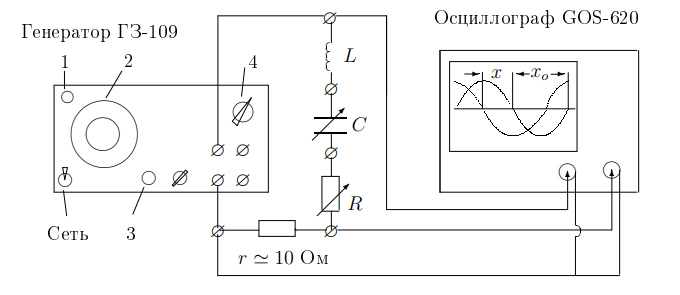
\includegraphics[width=0.7\linewidth]{scheme}
		\caption{Экспериментальная установка}
		\label{fig:scheme}
	\end{figure}
	\section{Ход работы}
	\subsection{RC-цепь}
	Параметры установки следующие: ёмкость конденсатора C = 0.5 мкФ, сопротивление
	r = 12.4 Ом, частота источника $\nu$ = 1000 Гц. Модуль реактивного сопротивления равен: $X_1 = \frac{1}{\omega C} = 318.5$ Ом.
	Измерим зависимость сдвига фаз от R в диапазоне R от 0 Ом до 3200 Ом. Для этого будем
	измерять сдвиг x одной синусоиды относительно другой в делениях экрана осцилографа
	и половину периода одной из синусоид x0. Для повышения точности, будем увеличивать синусоиду, дабы лучше разрешить сдвиг. Для R = 800-1600 Ом увеличим ширину вдвое, Для R = >1600 Ом увеличим еще вдвое. Для упрощения визуальной оценки приведем x к близким значениям.
	\begin{table}[H]
		\centering
		\begin{tabular}{|c|c|c|c|c|c|}
			\hline
			R, Ом & $x_0$, дел & $x$, дел   & $\Delta x$, дел   & $\psi$, рад  & $\Delta \psi$, рад \\ \hline
			0     & 2.5 & 1.20 & 0.10 & 1.51 & 0.13 \\ \hline
			400   & 2.0 & 0.50 & 0.10 & 0.79 & 0.16 \\ \hline
			800   & 2.5 & 0.30 & 0.05 & 0.38 & 0.06 \\ \hline
			1200  & 2.5 & 0.20 & 0.05 & 0.25 & 0.06 \\ \hline
			1600  & 2.5 & 0.20 & 0.05 & 0.25 & 0.06 \\ \hline
			2000  & 2.5 & 0.15 & 0.02 & 0.19 & 0.03 \\ \hline
			2400  & 2.5 & 0.10 & 0.02 & 0.13 & 0.03 \\ \hline
			2800  & 2.5 & 0.05 & 0.02 & 0.06 & 0.03 \\ \hline
			3200  & 2.5 & 0.05 & 0.02 & 0.06 & 0.03 \\ \hline
		\end{tabular}
		\caption{Зависимость сдвига фаз от сопротивления RC-цепи}
	\end{table}
	Согласно теории мы должны получить зависимость:
		\begin{equation*}
			 tan(\psi) = \frac{1}{\omega C R_{sum}}, f(x): k = 1
		\end{equation*}	
	\begin{table}[H]
		\centering
		\begin{tabular}{|c|c|c|c|c|c|c|c|c|c|}
			\hline
			$tan(\psi)$   & 15.89 & 1.00 & 0.40 & 0.26 & 0.26 & 0.19 & 0.13 & 0.06 & 0.06 \\ \hline
			$\Delta tan(\psi)$  & 1.32  & 0.20 & 0.07 & 0.06 & 0.06 & 0.03 & 0.03 & 0.03 & 0.03 \\ \hline
			$1/\omega C R_{sum}$ & 25.67 & 0.77 & 0.39 & 0.26 & 0.20 & 0.16 & 0.13 & 0.11 & 0.10 \\ \hline
		\end{tabular}
		\caption{Данные для построения графика $tan(\psi) = f(1/\omega C R_{sum})$}
	\end{table}
	На Рис.2 не будем отображать точку соответствующую R = 0 Ом, так как расстояние до нее много больше ширины графика если исключить эту точку, поэтому это мешает проводить оценку графика.
	\begin{figure}[H]
		\centering
		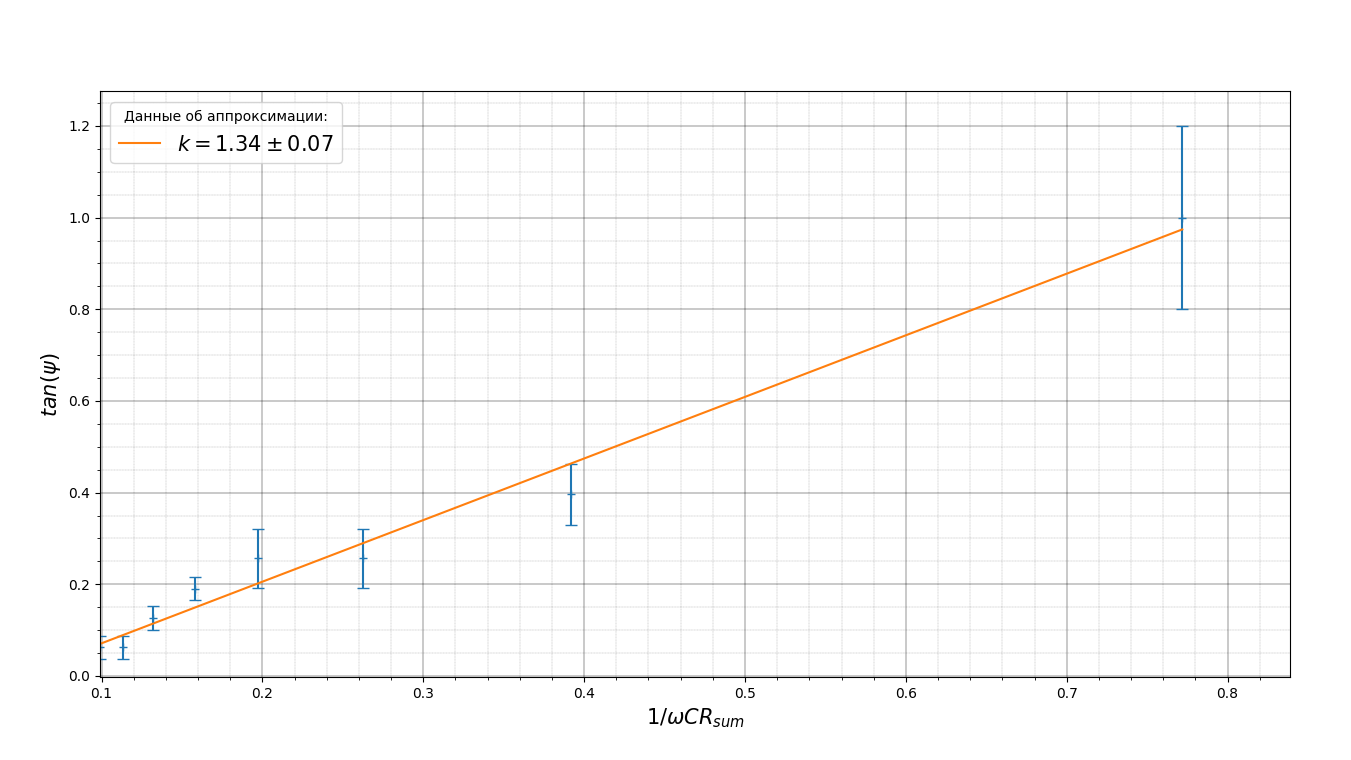
\includegraphics[width=0.9\linewidth]{RC}
		\caption{Зависимость $tan(\psi) = f(1/\omega C R_{sum})$}
		\label{fig:rc}
	\end{figure}
	\subsection{RL-цепь}
	Аналогично RC-цепи проведем замеры и запишем полученные данные в Таблицу 3. Реактивное сопротивление: $X_2 = \omega L = 314$ Ом
	\begin{table}[H]
		\centering
		\begin{tabular}{|c|c|c|c|c|c|}
			\hline
		R, Ом & $x_0$, дел & $x$, дел   & $\Delta x$, дел   & $\psi$, рад  & $\Delta \psi$, рад \\ \hline
			0     & 2.5 & 1.20 & 0.10 & 1.51 & 0.13 \\ \hline
			400   & 2.5 & 0.50 & 0.10 & 0.63 & 0.13 \\ \hline
			800   & 2.5 & 0.30 & 0.05 & 0.38 & 0.06 \\ \hline
			1200  & 2.5 & 0.20 & 0.05 & 0.25 & 0.06 \\ \hline
			1600  & 2.5 & 0.20 & 0.05 & 0.25 & 0.06 \\ \hline
			2000  & 2.5 & 0.15 & 0.02 & 0.19 & 0.03 \\ \hline
			2400  & 2.5 & 0.10 & 0.02 & 0.13 & 0.03 \\ \hline
			2800  & 2.5 & 0.05 & 0.02 & 0.06 & 0.03 \\ \hline
			3200  & 2.5 & 0.05 & 0.02 & 0.06 & 0.03 \\ \hline
		\end{tabular}
		\caption{Зависимость сдвига фаз от сопротивления RL-цепи}
	\end{table}
	Аналогично п. 3.1 не наносим на график точку соответствующую R = 0 Ом.
	\begin{table}[H]
		\centering
		\begin{tabular}{|c|l|l|l|l|l|l|l|l|l|}
			\hline
			$tan(\psi)$  & 15.89 & 0.73 & 0.40 & 0.26 & 0.26 & 0.19 & 0.13 & 0.06 & 0.06 \\ \hline
			$\Delta tan(\psi)$ & 1.32  & 0.15 & 0.07 & 0.06 & 0.06 & 0.03 & 0.03 & 0.03 & 0.03 \\ \hline
			$\omega L / R_{sum}$ & 6.94  & 0.71 & 0.37 & 0.25 & 0.19 & 0.15 & 0.13 & 0.11 & 0.10 \\ \hline
		\end{tabular}
		\caption{Данные для построения графика $tan(\psi) = f(\omega L / R_{sum})$}
	\end{table}
	
	\begin{figure}[H]
		\centering
		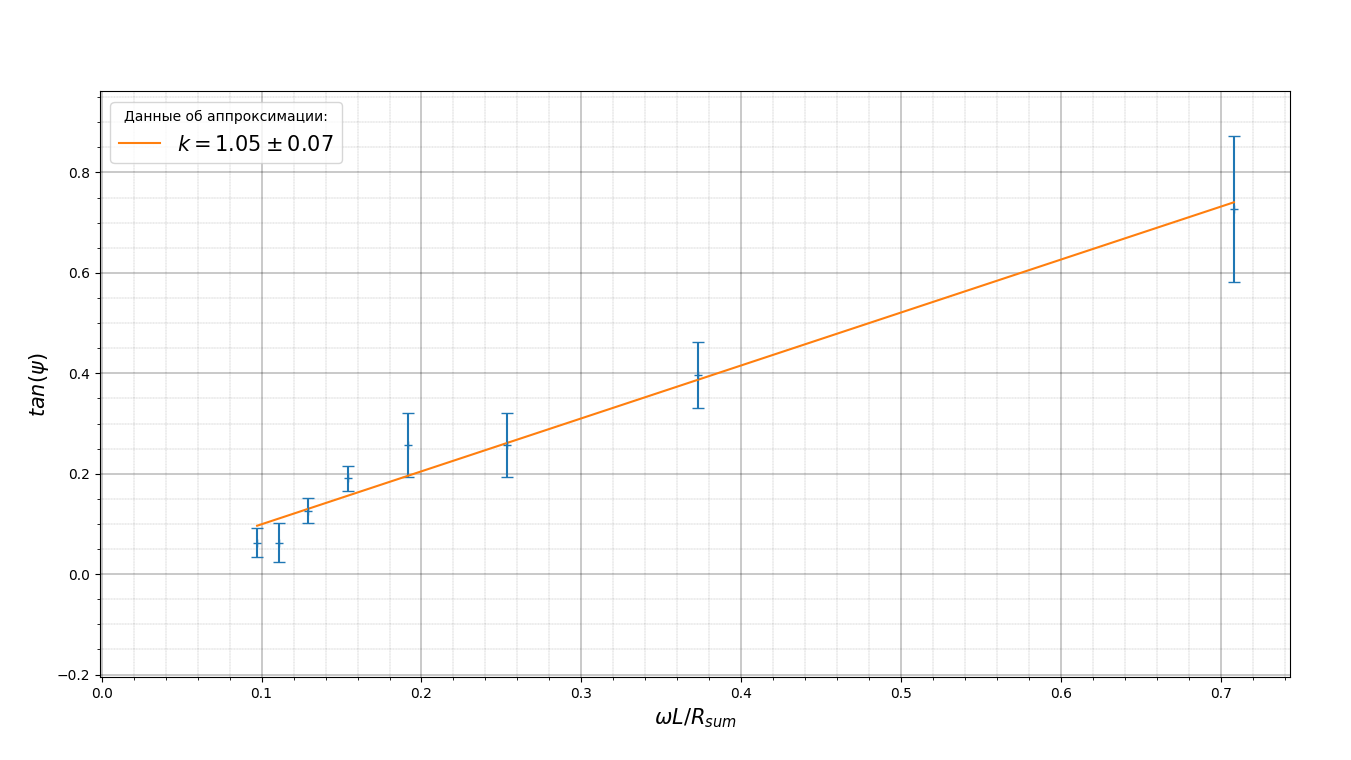
\includegraphics[width=0.9\linewidth]{RL}
		\caption{Зависимость $tan(\psi) = f(\omega L / R_{sum})$}
		\label{fig:rl}
	\end{figure}
	\subsection{RLC-цепь}
	Для RLC-цепи определим частоту резонанса (С = 0.5 мкФ, r = 12.4 Ом, L = 50.002 мГн):
	\begin{equation*}
		\nu_0 = \frac{1}{2\pi \sqrt{LC}} = 1007~ Гц
	\end{equation*}	
	\begin{table}[H]
		\centering
		\begin{tabular}{|cccc|cccc|}
			\hline
			\multicolumn{4}{|c|}{R   = 0 Ом}                                                         & \multicolumn{4}{c|}{R = 100 Ом}                                                        \\ \hline
			\multicolumn{1}{|c|}{$\nu$, Гц}   & \multicolumn{1}{c|}{$x_0$} & \multicolumn{1}{c|}{$x$}    & $|\psi|$  & \multicolumn{1}{c|}{$\nu$, Гц}   & \multicolumn{1}{c|}{$x_0$} & \multicolumn{1}{c|}{$x$}   & $|\psi|$  \\ \hline
			\multicolumn{1}{|c|}{870}  & \multicolumn{1}{c|}{2.9} & \multicolumn{1}{c|}{1}    & 1.08 & \multicolumn{1}{c|}{800}  & \multicolumn{1}{c|}{3.1} & \multicolumn{1}{c|}{0.8} & 0.81 \\ \hline
			\multicolumn{1}{|c|}{900}  & \multicolumn{1}{c|}{2.8} & \multicolumn{1}{c|}{0.9}  & 1.01 & \multicolumn{1}{c|}{850}  & \multicolumn{1}{c|}{3}   & \multicolumn{1}{c|}{0.6} & 0.63 \\ \hline
			\multicolumn{1}{|c|}{930}  & \multicolumn{1}{c|}{2.7} & \multicolumn{1}{c|}{0.6}  & 0.70 & \multicolumn{1}{c|}{900}  & \multicolumn{1}{c|}{2.8} & \multicolumn{1}{c|}{0.4} & 0.45 \\ \hline
			\multicolumn{1}{|c|}{960}  & \multicolumn{1}{c|}{2.6} & \multicolumn{1}{c|}{0.4}  & 0.48 & \multicolumn{1}{c|}{950}  & \multicolumn{1}{c|}{2.5} & \multicolumn{1}{c|}{0.2} & 0.25 \\ \hline
			\multicolumn{1}{|c|}{1000} & \multicolumn{1}{c|}{2.5} & \multicolumn{1}{c|}{0.05} & 0.06 & \multicolumn{1}{c|}{1000} & \multicolumn{1}{c|}{2.5} & \multicolumn{1}{c|}{0}   & 0.00 \\ \hline
			\multicolumn{1}{|c|}{1030} & \multicolumn{1}{c|}{2.4} & \multicolumn{1}{c|}{0.4}  & 0.52 & \multicolumn{1}{c|}{1050} & \multicolumn{1}{c|}{2.4} & \multicolumn{1}{c|}{0.2} & 0.26 \\ \hline
			\multicolumn{1}{|c|}{1060} & \multicolumn{1}{c|}{2.4} & \multicolumn{1}{c|}{0.6}  & 0.79 & \multicolumn{1}{c|}{1100} & \multicolumn{1}{c|}{2.4} & \multicolumn{1}{c|}{0.4} & 0.52 \\ \hline
			\multicolumn{1}{|c|}{1090} & \multicolumn{1}{c|}{2.3} & \multicolumn{1}{c|}{0.7}  & 0.96 & \multicolumn{1}{c|}{1150} & \multicolumn{1}{c|}{2.2} & \multicolumn{1}{c|}{0.6} & 0.86 \\ \hline
		\end{tabular}
	\caption{Сдвиг фаз в RLC-цепи}
	\end{table}
	
	\begin{table}[H]
		\centering
		\begin{tabular}{|lcccccccc|}
			\hline
			\multicolumn{9}{|c|}{R=0   Ом}                                                                                                                                                                                                           \\ \hline
			\multicolumn{1}{|l|}{$|\psi|/\pi$}  & \multicolumn{1}{c|}{0.34} & \multicolumn{1}{c|}{0.32} & \multicolumn{1}{c|}{0.22} & \multicolumn{1}{c|}{0.15} & \multicolumn{1}{c|}{0.02} & \multicolumn{1}{c|}{0.17} & \multicolumn{1}{c|}{0.25} & 0.30 \\ \hline
			\multicolumn{1}{|l|}{$\nu/\nu_0$} & \multicolumn{1}{c|}{0.86} & \multicolumn{1}{c|}{0.89} & \multicolumn{1}{c|}{0.92} & \multicolumn{1}{c|}{0.95} & \multicolumn{1}{c|}{0.99} & \multicolumn{1}{c|}{1.02} & \multicolumn{1}{c|}{1.05} & 1.08 \\ \hline
			\multicolumn{9}{|c|}{R = 100 Ом}                                                                                                                                                                                                         \\ \hline
			\multicolumn{1}{|l|}{$|\psi|/\pi$}  & \multicolumn{1}{c|}{0.26} & \multicolumn{1}{c|}{0.20} & \multicolumn{1}{c|}{0.14} & \multicolumn{1}{c|}{0.08} & \multicolumn{1}{c|}{0.00} & \multicolumn{1}{c|}{0.08} & \multicolumn{1}{c|}{0.17} & 0.27 \\ \hline
			\multicolumn{1}{|l|}{$\nu/\nu_0$} & \multicolumn{1}{c|}{0.79} & \multicolumn{1}{c|}{0.84} & \multicolumn{1}{c|}{0.89} & \multicolumn{1}{c|}{0.94} & \multicolumn{1}{c|}{0.99} & \multicolumn{1}{c|}{1.04} & \multicolumn{1}{c|}{1.09} & 1.14 \\ \hline
		\end{tabular}
	\caption{Данные для построения графика $|\psi|/\pi = f(\nu/\nu_0)$}
	\end{table}
	Построим на одном графике сдвиг фаз в единицах $\pi$ для R = 0 Ом и R = 100 Ом. Использовали большую развертку, значит $\Delta \psi = 0.02$.
	\begin{figure}[H]
		\centering
		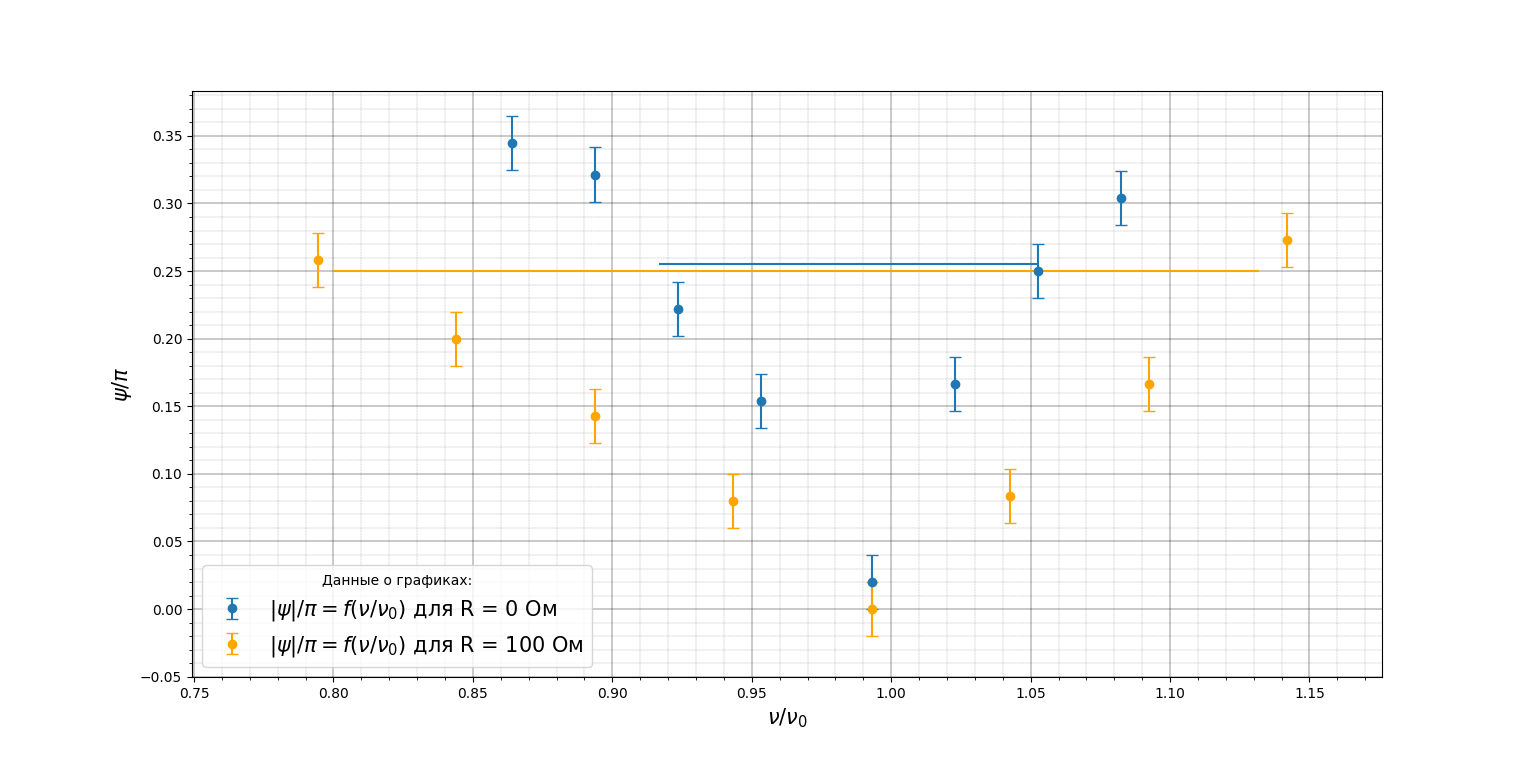
\includegraphics[width=0.9\linewidth]{RLC}
		\caption{Зависимость $|\psi|/\pi = f(\nu/\nu_0)$}
		\label{fig:rlc}
	\end{figure}
	
	Рассчитаем добротность экспериментально:\\
	\begin{equation*}
		Q =\frac{\nu_0}{2\Delta \nu};		
		~Q_0 = 6.9 \pm 1.8; Q_{100} = 3.0 \pm 0.4
	\end{equation*}	
	Рассчитаем добротность теоретически:\\
	\begin{equation*}
		Q =\frac{1}{R}\sqrt{\frac{L}{C}};		
		~Q_0 = 6.8; Q_{100} = 2.2
	\end{equation*}	
	\subsection{Фазовращатель}
	Нарисуем векторную диаграмму для случая $\psi = \pi / 2$:
	\begin{figure}[H]
		\centering
		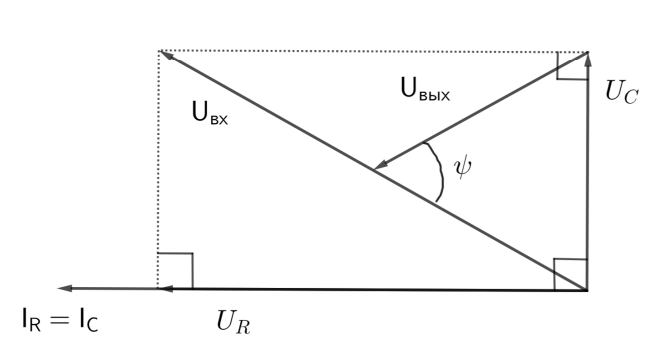
\includegraphics[width=0.8\linewidth]{phase}
		\caption{Векторная диаграмма для $\psi = \pi / 2$ }
		\label{fig:phase}
	\end{figure}
	По расчетам получим: $R = 318.5 ~Ом$, на практике получили значение:$R = 330\pm 10~ Ом$. Погрешность при практическом измерении оценена как шаг дискретизации (поворот какой-либо из ручек магазина), при котором отсутствуют заметные глазу изменения на осциллографе.
	\section{Выводы}
	1)В работе проверили справедливость теоретических соображений о зависимости сдвига фаз от параметров системы. Для RC-цепи $k = 1.34\pm 0.07$, RL-цепи $k = 1.05\pm 0.07$, эталонный к равен единице.\\
	2)Для RLC-цепи проверили рассчитали добротность колебаний (см. п. 3.3), практические результаты совпали с теорией, с учетом погрешности.\\
	3)Рассчитали значение резонансного сопротивления, получили данные значения на практике.
	
\end{document}
